\begin{figure}[h!]
     \centering
     \begin{subfigure}[b]{0.3\textwidth}
         \centering
         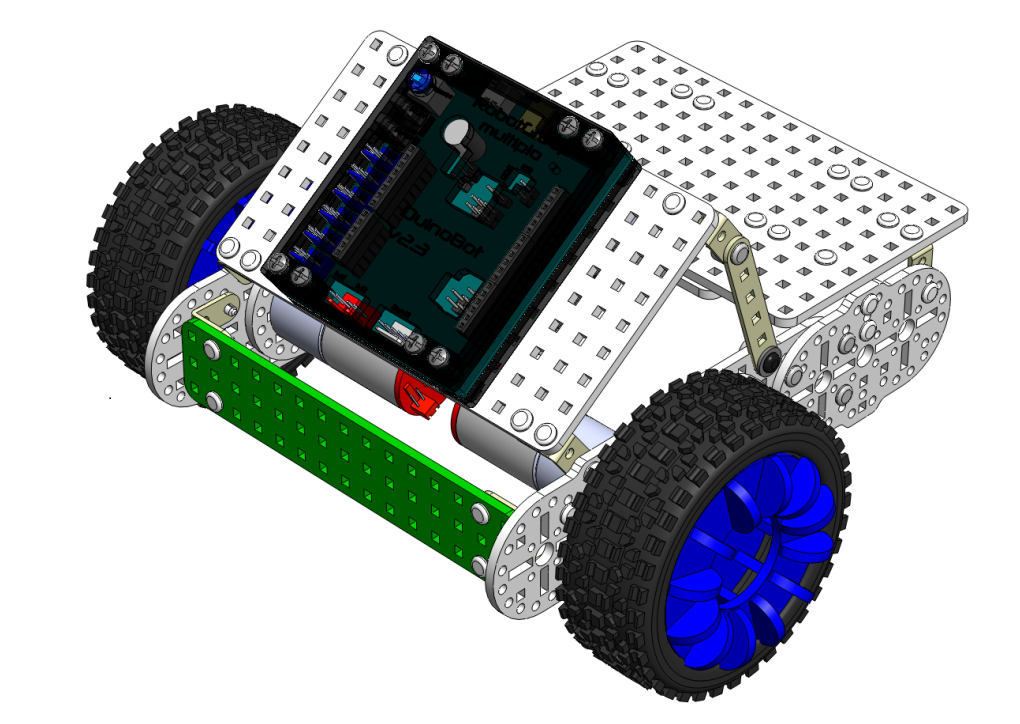
\includegraphics[width=\textwidth]{robot}
         \caption*{ Robot}
         \label{fig:robot}
     \end{subfigure}
     \hfill
     \begin{subfigure}[b]{0.3\textwidth}
         \centering
         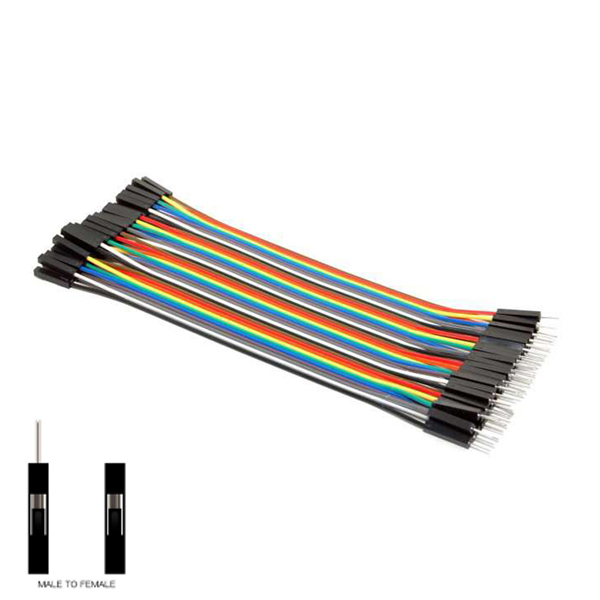
\includegraphics[width=\textwidth]{jumper}
         \caption*{ 4 Adet Erkek-Di�i Jumper}
         \label{fig:kumanda}
     \end{subfigure}
     \hfill
     \begin{subfigure}[b]{0.3\textwidth}
         \centering
         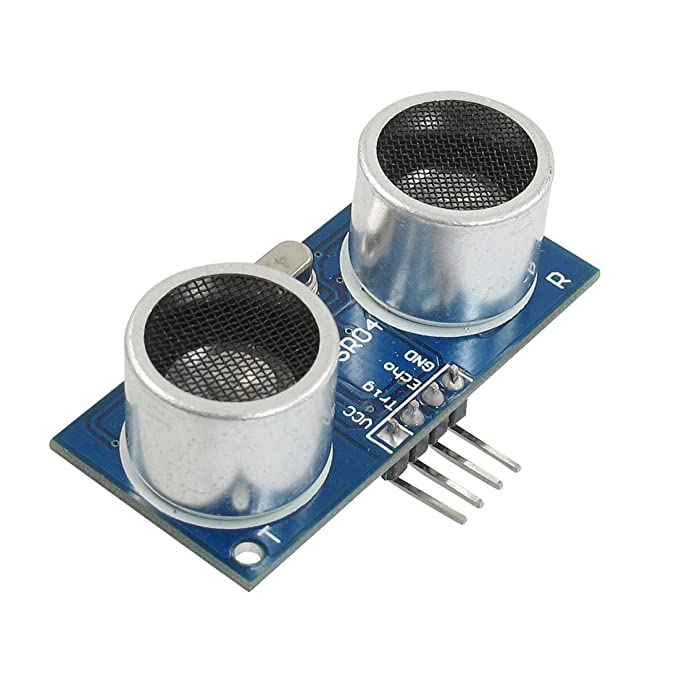
\includegraphics[width=\textwidth]{sens}
         \caption*{ Kablo}
         \label{fig:cable}
     \end{subfigure}
      \caption{�kinci uygulamada kulland���m�z malzemeler}
\end{figure}

\section{SONU�LAR VE �NER�LER}
G�n�m�zde robotik sekt�r� b�y�k bir h�zla b�y�yor. Bu nedenle bu projenin �nemi, ��rencileri bu sekt�re temel bilgilerle tan��t�rarak bu sekt�rde g�ncel olabilmelerini sa�lamakt�r.

Bu projede yapt���m�z uygulamalar �ok esnektir ve ��rencilere de�i�iklik yapma esnekli�i verir ve istedikleri algoritmay� uygulayabilirler.
